\documentclass[12pt]{article}
\usepackage{times}
\usepackage{import}
\usepackage{geometry}
\usepackage{svg}
\usepackage{amsmath}
\usepackage{float}
\usepackage{caption}
\usepackage{subcaption}
\usepackage{graphicx,xcolor}
\geometry{letterpaper, portrait, margin=1in}
\usepackage[utf8]{inputenc}
\usepackage{enumitem,amssymb}
\usepackage{ragged2e}
\newlist{thematic}{itemize}{8}
\setlist[thematic]{label=$\square$}
\usepackage{pifont}
\newcommand{\cmark}{\ding{51}}%
\newcommand{\xmark}{\ding{55}}%
\renewcommand\labelitemi{$\cdot$}
\newcommand{\done}{\rlap{$\square$}{\raisebox{2pt}{\large\hspace{1pt}\cmark}}%
\hspace{-2.5pt}}
\newcommand{\wontfix}{\rlap{$\square$}{\large\hspace{1pt}\xmark}}

\begin{document}
\raggedright
\huge
REG - F19 - Porteføjle 1 \linebreak
\normalsize


\subsection*{System Modeling}
\begin{itemize}
  \item Setup a model (nth-order dierential equation) of the system.
  \item Derive a linearized model of the system at an angle of $\pi/3$ rad.
\end{itemize}

\subsection*{Performance Specification}

\begin{itemize}
  \item Specify a desired performance of the system.
\end{itemize}
The chosen performance specifications are as following:
\begin{itemize}
  \item Rise time = 1.0 seconds.
  \item Settling time = 1.2 seconds.
  \item Overshoot = 2 procent.
\end{itemize}
 The following specifications has been chosen based on the system being a robotic arm. It should neither have too fast nor too slow a rise time or settling time. If the rise time is too slow, it'll limit its usPerformancePerformancee significantly however if it moves too quickly it might both be impossible due to the motor physical limits and very dangerous for people working around and with it. The settling time and overshoot both should be as low as possible.
\subsection*{Controller Design}
\begin{itemize}
  \item Design a PID controller for the linearized model of the system such that it attains the desired performance. The tuning procedure should be described.
\end{itemize}

Our transferfunction is as following and is devived from the linearized model:
\begin{equation} \label{G_s}
  G(s) = \frac{3}{s^2 + 0.3s -7.365}
\end{equation}
First the poles of the systemet is found to be $2.568$ and $-2.8680$ respectively.\\
To design the PID controller there will be made use of root locus plots to observe the behaviour of the system and to add zeros to obtain the desired behaviour. A PID controller consists of 3 parts, a gain part P, an integral of the error which corrects the steady state error part I and a D part. The D and I part both adds a zero to the transfer function. This is very useful if the transferfunction for K(s) can be rewritten from it's original form, see equation \ref{k_s_original}, to a more manageable form, see equation \ref{k_s_rewritten}.
\begin{equation} \label{k_s_original}
  kp\cdot(1+\frac{1}{Ti}\cdot \frac{1}{s}+Tds)
\end{equation}
\begin{equation} \label{k_s_rewritten}
  kp\cdot(\frac{Tds^2 + s + \frac{1}{Ti}}{s})
\end{equation}
However due to the equation above we will add an extra pole as well as two zeroes. It'd be useful to cancel out one of the poles with one of the zeros. As the first iteration the desired zeroes position is (-1,0) and (-2.568), where we cancel out pole (-2.868), which results in a $Ti = 0.146$ and $Td = 0.60$. Kp will be adjusted through the tuning but starts on $6.68$.\\
The root locus plot of this looks like this:
\begin{figure}[H]
  \centering
  \def\svgwidth{\textwidth}
  \import{./Matlab/images/}{matlab_rlocus.pdf_tex}
  \caption{Root locus plot} \label{my_root_locus_plot}
\end{figure}
Next up is checking the performance of the entire system, see transferfunction \ref{closed_loop_system}.
\begin{equation} \label{closed_loop_system}
    T(s) = \frac{K(s) \cdot G(s)}{1+K(s)\cdot G(s)}
\end{equation}
By using the matlab function stepinfo and step, both the step responds and the information of the system can be concluded. The results with $Ti = 0.146$, $Td = 0.60$ and $kp = 6.68$ gave a unstable system not worth mentioning, but by increasing the gain Kp to $20.00$ the following was observed:
\begin{itemize}
  \item RiseTime: 0.1135s
  \item SettlingTime: 1.2523s
  \item SettlingMin: 0.9371
  \item SettlingMax: 1.4381
  \item Overshoot: 43.8123
  \item Peak: 1.4381
\end{itemize}
\begin{figure}[H]
  \centering
  \def\svgwidth{0.5\textwidth}
  \import{./Matlab/images/}{kp_20_step.pdf_tex}
  \caption{step response for the first iteration} \label{my_first_step}
\end{figure}
Next the Kp increases to $40.00$ and the following performance of the system can be observed:
\begin{itemize}
  \item RiseTime: 0.0727
  \item SettlingTime: 0.6485
  \item SettlingMin: 0.9097
  \item SettlingMax: 1.2489
  \item Overshoot: 24.8889
  \item Peak: 1.2489
\end{itemize}
\begin{figure}[H]
  \centering
  \def\svgwidth{0.5\textwidth}
  \import{./Matlab/images/}{kp_40_step.pdf_tex}
  \caption{step response for the second iteration} \label{my_second_step}
\end{figure}
The performance has technically inproved when it comes to rise time and settling time, however the desired rise time is around 1 second so it isn't an improvemnt for the desired system. The overshoot has decreased significantly with $50\%$ which is a huge improvement. Still, however, far from the desired 1\%. The steady state error is eliminated as the previous with try, observed on figure \ref{my_second_step}. This time the Kp has increased to $60.00$.
\begin{itemize}
  \item RiseTime: 0.0547
  \item SettlingTime: 0.6075
  \item SettlingMin: 0.9268
  \item SettlingMax:  1.1780
  \item Overshoot: 17.8013
  \item Peak: 1.1780
\end{itemize}
\begin{figure}[H]
  \centering
  \def\svgwidth{0.5\textwidth}
  \import{./Matlab/images/}{kp_60_step.pdf_tex}
  \caption{step response for the third iteration} \label{my_third_step}  
\end{figure}
As observed with the previous tries the rise time and overshoot has decreased significantly again, still not enough to reach our desired 1\% overshoot. The rise time is way too fast and decreasing with Kp increasing, so increasing the kp will not improve our system anymore. \\
This is realistically not going to work with the properties of the motor. We have decided to go with a $Kp = 60.00$ and simulate that. In hindersight, we should try changing the zeroes by tuning the I and D.


\subsection*{Simulation}

\begin{itemize}
  \item Simulate the linearized system with set point $\pi/3$ rad. and initial condition 0 rad.
  \item Simulate the nonlinear system model with the designed PID control.
\end{itemize}

\begin{figure}[H]
\centering
\begin{subfigure}{0.5\textwidth}
  \centering
  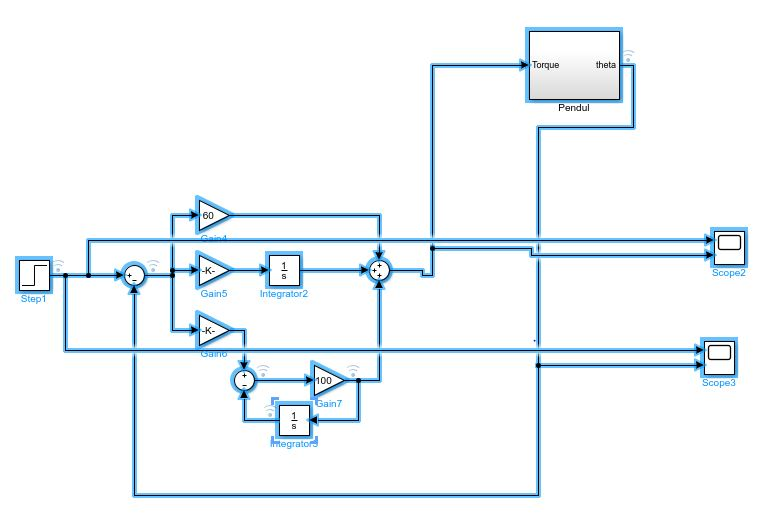
\includegraphics[width=1\linewidth]{images/ulin_simu.jpg}
  \caption{the input of step response of the simulated linearized system} \label{my_input_step_li}
\end{subfigure}%
\begin{subfigure}{0.5\textwidth}
  \centering
  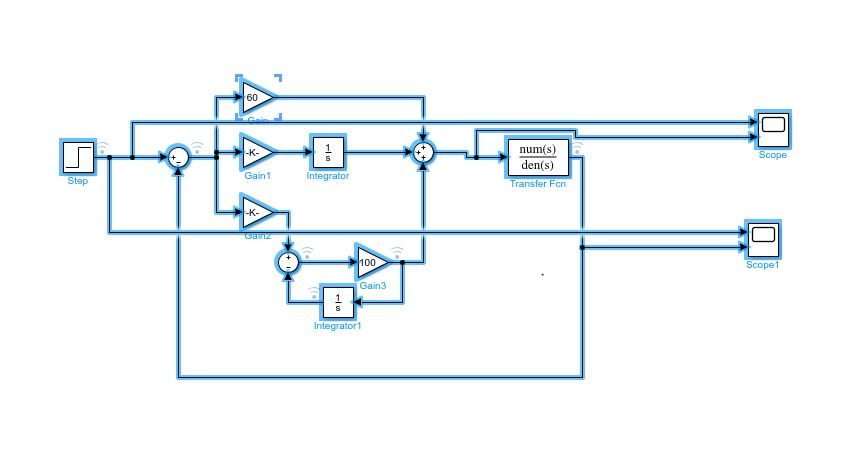
\includegraphics[width=1\linewidth]{images/lin_simu.jpg}
  \caption{the output of the step response of the simulated linearized system} \label{my_output_step_li}
\end{subfigure}
\caption{A figure that shows the step response input and output of the simulated linearized system.}
\label{fig:step_li}
\end{figure}

The linearized system has been simulated below and shows that

\begin{figure}[H]
\centering
\begin{subfigure}{0.5\textwidth}
  \def\svgwidth{\textwidth}
  \import{./Matlab/images/}{sim_unlin_input.pdf_tex}
  \label{}
  \centering
  \caption{the input of step response of the simulated linearized system} \label{my_input_step_li}
\end{subfigure}%
\begin{subfigure}{0.5\textwidth}
  \centering
  \def\svgwidth{\textwidth}
  \import{./Matlab/images/}{sim_unlin_output.pdf_tex}
  \caption{the output of the step response of the simulated linearized system} \label{my_output_step_li}
\end{subfigure}
\caption{A figure that shows the step response input and output of the simulated linearized system.}
\label{fig:step_li}
\end{figure}

Here the nonlinear system shows a little bit less overshoot than the linearized system. It shows that the output is equal to the expected


\begin{figure}

\end{figure}








\end{document}
